%----------------------------------------------------------------------------------------
%	PACKAGES AND DOCUMENT CONFIGURATIONS
%----------------------------------------------------------------------------------------
\documentclass[11pt]{article}
\usepackage{amsmath} % Required for some math elements
\usepackage{hyperref} 
\usepackage{xcolor}
\usepackage{lipsum} 
\usepackage{cite}
\usepackage{graphicx} % Required for the inclusion of images
\usepackage{algorithmic}
\usepackage{array}
\usepackage{bookmark}
\usepackage{listings}
\usepackage{amssymb}
\usepackage{enumitem}
\usepackage{pythonhighlight}
\usepackage[T1]{fontenc}
\usepackage{inconsolata}
\usepackage[margin=8mm]{geometry}
\usepackage[caption=false, font=footnotesize]{subfig}
\usepackage{fancyhdr}
\pagestyle{fancy}
\renewcommand{\headrulewidth}{0.4pt}
\renewcommand{\footrulewidth}{0.4pt}

\usepackage[active,tightpage]{preview}
\renewcommand{\PreviewBorder}{1in}
\newcommand{\Newpage}{\end{preview}\begin{preview}}
  


\newlist{steps}{enumerate}{1}
\setlist[steps, 1]{label = Step \arabic*:}

\hypersetup{ %color attributes of citation, link, etc.
    colorlinks=true,
    linkcolor=blue,
    filecolor=gray,      
    urlcolor=blue,
    citecolor=blue,
}

\newcommand{\matlab}{\textsc{Matlab }} %very important and totally necessary addition
\newcommand{\hdotrule}[1]{\hbox to \textwidth{\leaders\hbox to #1pt{\hss . \hss}\hfil}}

\newcommand\Item[1][]{%
  \ifx\relax#1\relax  \item \else \item[#1] \fi
  \abovedisplayskip=0pt\abovedisplayshortskip=0pt~\vspace*{-\baselineskip}}
%----------------------------------------------------------------------------------------
%	DOCUMENT INFORMATION
%----------------------------------------------------------------------------------------

\title{ECEN 405 \\ Lab 5: Power converters \\ (Part 4 - Buck-Boost Converter) Submission}
\author{Daniel Eisen : 300447549}
\date{\today}

\begin{document}
\begin{preview}

    \maketitle
    \hrule
    %----------------------------------------------------------------------------------------
    %	DOCUMENT CONTENT
    %----------------------------------------------------------------------------------------
    \section{Design}
    $V_d=10V,\; R_L=500\Omega,\; L=4mH,\; C=100\mu F,\; D=0.6, D_{max} = 0.67$
        \subsection*{Switching Frequency}
            $$V_{o}=\frac{D}{1-D}V_{d}=15V$$
            $$I_{o}=\frac{V_{o}}{R_{L}}=0.03A$$
            $$I_{ripple}=0.2I_{o}\frac{V_{o}}{V_{d}}=0.009A$$
            $$I_{omax}=I_{o}+0.5I_{ripple}=0.0345A$$
            $$f_{sw}=\frac{V_{d}\left(V_{o}-V_{d}\right)}{LI_{ripple}V_{o}} = 92592.5925926Hz$$
            \begin{center}
                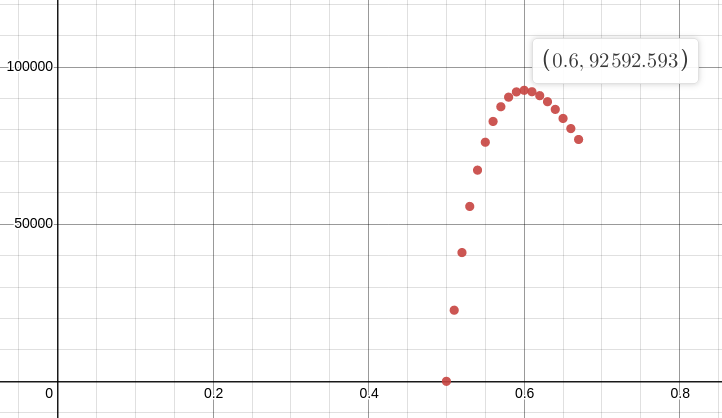
\includegraphics[width=0.5\textwidth]{img/fw_d.png}\\
                \textit{Duty Cycle vs Switching Frequency}
            \end{center}
            Note that a 60\% duty cycle requires the highest switching frequency.
        \subsection*{Schematic}
        \begin{center}
            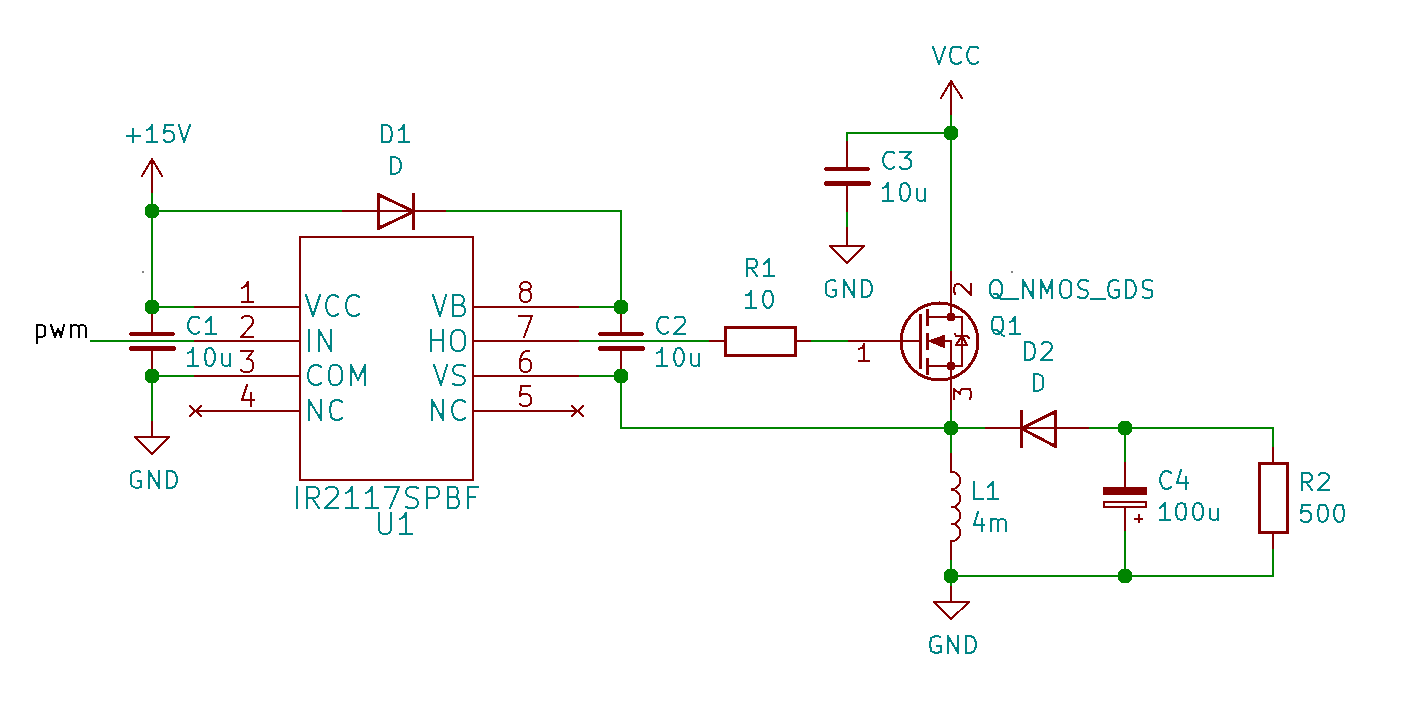
\includegraphics[width=\textwidth]{img/schem.png}
        \end{center}
        \subsection*{Output Voltage Ripple}
            $$V_{ripple}=\frac{I_{omax}D_{max}}{f_{sw}C}=0.00425V$$
    \section{Output}
    The USB drive with the "real" screenshots are still in the lab plugged into the computer with a half written report on it. So here is what it remember the signal looking like in paint. 
        \begin{center}
            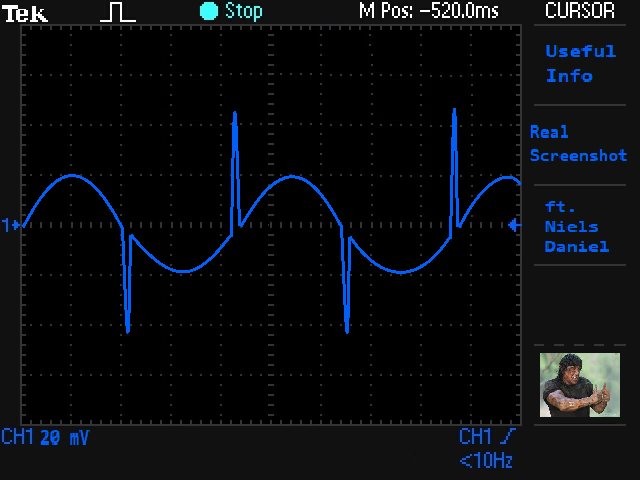
\includegraphics[width=\textwidth]{img/out.png}
        \end{center}
        From memory we had a ripple voltage or around 40mV to 80mV.
    \section{Efficiency}
        \begin{center}
            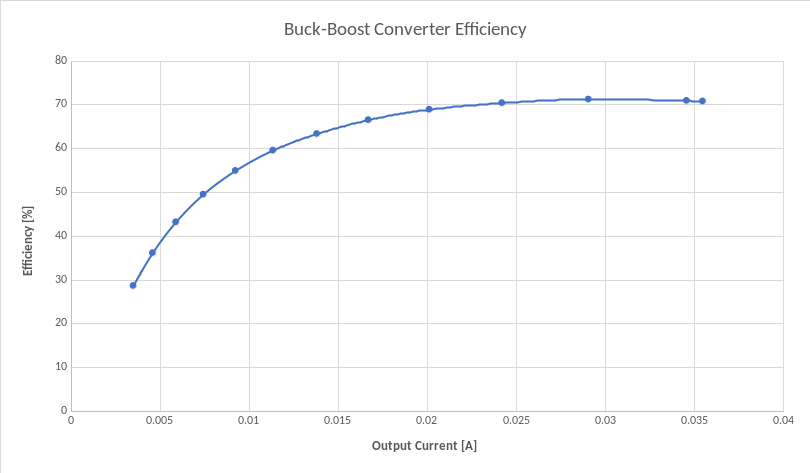
\includegraphics[width=\textwidth]{img/eff.png}
        \end{center}
    \hrule
\end{preview}
\end{document}